\documentclass{beamer}
\usepackage{etex} % fixes new-dimension error
\usepackage{lmodern}
\usepackage[T1]{fontenc}
\usepackage[absolute,overlay]{textpos} % this is for textblock
\usepackage{tikz}
\usetikzlibrary{arrows.meta, calc, fit, tikzmark}
\usepackage{pgfplots}
\usepackage{multicol}
\usepackage{proof}
\usepackage{hyperref}
\usepackage{array} % m in tabularalso


%-------------- template --------------------------------------------------
\usetheme{metropolis}
\metroset{block=fill}
%\usetheme{Boadilla}

% Configuring the foot line
\setbeamertemplate{footline}
{
  \leavevmode%
  \hbox{%
  \begin{beamercolorbox}[wd=.4\paperwidth,ht=2.25ex,dp=1ex,center]{author in head/foot}%
    \usebeamerfont{author in head/foot}\insertshortauthor
  \end{beamercolorbox}%
  \begin{beamercolorbox}[wd=.5\paperwidth,ht=2.25ex,dp=1ex,center]{title in head/foot}%
    \usebeamerfont{title in head/foot}\insertsection
  \end{beamercolorbox}%
  \begin{beamercolorbox}[wd=.1\paperwidth,ht=2.25ex,dp=1ex,right]{date in head/foot}%
    \insertframenumber{} / \inserttotalframenumber\hspace*{2ex} 
  \end{beamercolorbox}}%
  \vskip0pt%
}
% No configuration symbols
\setbeamertemplate{navigation symbols}{}
%----------------------------------------------------------------------------

% context
\AtBeginSection[]
{
    \begin{frame}
        \frametitle{Table of Contents}
        \tableofcontents[currentsection]
    \end{frame}
}
\author[Renato Neves]{Renato Neves}
% logos of institutions
\titlegraphic{
  \begin{textblock*}{5cm}(6.7cm,7.57cm)
     \includegraphics[scale=0.05525]{images/uminho.png}
  \end{textblock*}
  \begin{textblock*}{5cm}(9.4cm,7.57cm)
    \includegraphics[scale=0.50]{images/haslab.pdf}
  \end{textblock*}
}
% No date
\date{}


%----------------------------------------------------------------------------
\usepackage{graphicx,amsmath}
\usepackage{stmaryrd} % cf. interleave
\usepackage{booktabs}
\usepackage{amscd}

\usepackage{alltt}
%------ using xy ------------------------------------------------------------
\usepackage[all]{xy}
%\def\larrow#1#2#3{\xymatrix{ #3 & #1 \ar[l] _-{#2} }}
\def\larrow#1#2#3{\xymatrix{ #3 & #1 \ar[l] _--{#2} }}
\def\rarrow#1#2#3{\xymatrix{ #1 \ar[r]^-{#2} & #3 }}
\def\arLaw#1#2#3#4#5{
\xymatrix{
        #1      \ar@/^1pc/[rr]^-{#4} &
        #5 &
        #2      \ar@/^1pc/[ll]^-{#3}
}}

\newcommand{\blue}[1]{\textcolor{blue}{#1}}
\begin{document}

\title{Hybrid Programming}

\frame[plain]{\titlepage}

\section{Overview}

\begin{frame}{Last Lectures}
       
       Explored a simple language (\textsc{ccs}) and its semantics

       Used it to design \alert{\underline{communicating}} systems

       Expanded this study to the \alert{\underline{timed}} setting
       
       Used this to save us all from zombies !!

\end{frame}

\begin{frame}{Going Beyond the Timed Setting}
        \begin{minipage}[0.3\textheight]{\textwidth}
        \begin{columns}[c]
                \begin{column}{0.45\textwidth}
                \scalebox{0.6}{
                  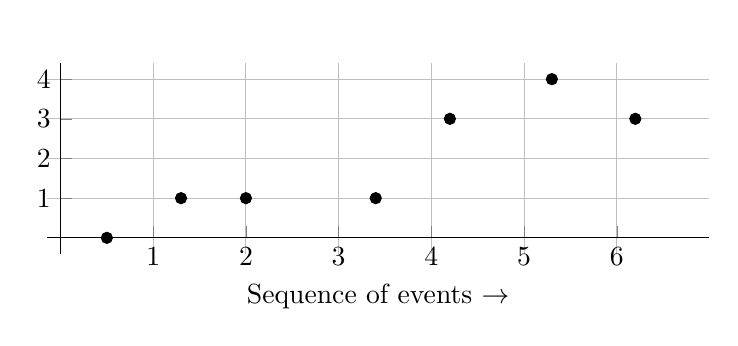
\begin{tikzpicture}
                   \begin{axis}[width=10cm, height=4cm, x axis line style={}, grid =
                     major, y axis line style={},
                     title={\textbf{}}, xlabel={\tikzmark{y1}\tikzmark{y2}Sequence
                     of events $\rightarrow$}, xtick =
                     {0,1,2,3,4,5,6}, xmax=7, axis lines*=center,
                     ytick={0,1,2,3,4,5,6},ylabel={},
                     xlabel near ticks, ylabel near ticks] \addplot [color=black,
                             only marks, domain = 0:5 ] 
                             coordinates {(0.5,0) (1.3,1) (2,1) (3.4,1) 
                             (4.2,3) (5.3,4) (6.2,3)};
                   \end{axis}
                  \end{tikzpicture}} 
                \end{column}
                \begin{column}{0.1\textwidth} 
                        \hspace{0.5cm} \textbf{+}                
                \end{column}
                \begin{column}{0.50\textwidth} 
                \scalebox{0.6}{ 
                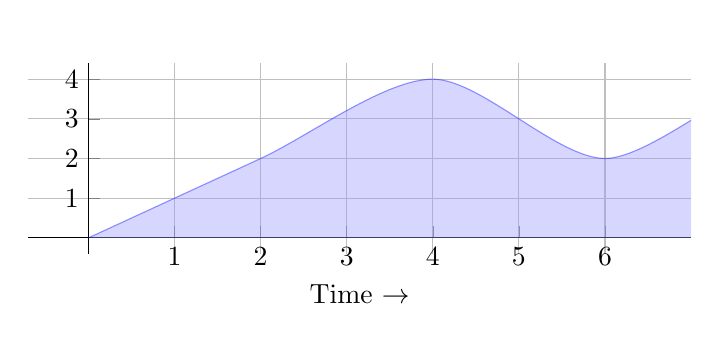
\begin{tikzpicture}
                \begin{axis}[width=10cm, height=4cm, x axis line style={}, grid =
                    major, y axis line style={},
                     title={\textbf{}}, xlabel={\tikzmark{x1}\tikzmark{x2}Time $\rightarrow$}				, xtick = {0,1,2,3,4,5,6} , xmax=7, axis lines*=center,
                     ytick={0,1,2,3,4,5,6}, ylabel={},
                     xlabel near ticks, ylabel near ticks] \addplot [color=blue, smooth,
                     domain = 0:5, fill = blue!40!white, opacity=0.4 ] coordinates {
                     (0,0) (2,2) (4,4) (6,2) (8,4) (8,0)};
                \end{axis}
                \end{tikzpicture}}
                \end{column}
        \end{columns}
        \end{minipage}

        \vspace{1.5cm}
        \begin{center}
                Computational devices now interact with \alert{\underline{arbitrary}}
                physical processes (and not just time)
        \end{center}

        \begin{tikzpicture}[overlay,remember picture,
box/.style = {rounded corners},
pin edge={-Stealth,thick, red}]
\coordinate (x1) at ($({pic cs:x1})+(-4ex, 1.5ex)$);
\coordinate (x2) at ($({pic cs:x2})+(-5ex,-0.5ex)$);
\node[semitransparent,
     fit=(x1) (x2),
     pin=below:\tiny{Described via differential equations}]  {};
\end{tikzpicture} \begin{tikzpicture}[overlay,remember picture, box/.style
= {rounded corners}, pin edge={-Stealth,thick, red}] \coordinate (y1) at
     ($({pic cs:y1})+(-0.5ex, 1.5ex)$); \coordinate (y2) at ($({pic
     cs:y2})+(-1.5ex,-0.5ex)$); \node[semitransparent, fit=(y1) (y2),
     pin=below:\tiny{Described via classical methods of computation}]
{};
\end{tikzpicture}


\end{frame}

\begin{frame}{Which language ?}

        This time we explore a simple, \alert{\underline{imperative
        language}}

        No concurrency and no communication

        \dots\ 
        languages with such features are still underdeveloped

        Perhaps some of you would like to improve them :-)

\end{frame}

\begin{frame}{The Hybrid While-Language}

        \vspace{0.7cm}
	\begin{block}{Linear Terms}
	$\mathtt{LTerm} \ni \tikzmark{r1} \mathtt{r} \tikzmark{r2} \mid \mathtt{r \cdot t}
        \mid \tikzmark{u1} \mathtt{x} \tikzmark{u2} \mid \mathtt{t + s}$
	\end{block}

	\vspace{0.7cm}
	\begin{block}{Atomic Programs}
	$\mathtt{At} \ni \mathtt{x := t} \mid
	\mathtt{x'_1 = t_1, \dots, x'_n = t_n \> \> \tikzmark{d1}\blue{for}\tikzmark{d2} 
	\> \> t }$
	\end{block}

	\vspace{0.7cm}
	\begin{block}{Programs}
	$\mathtt{Prog} \ni \mathtt{a} \mid
	\mathtt{p \> \blue{;} \> q} \mid
	\mathtt{\blue{if} \> b \> \blue{then} \> p \> \blue{else} \> q} \mid
	\mathtt{\blue{while} \> b \> \blue{do} \> \{ \> p \> \}}$
	\end{block}

	\begin{tikzpicture}[overlay,remember picture,
	box/.style = {rounded corners},
	pin edge={-Stealth,thick, red}]
	\coordinate (r1) at ($({pic cs:r1})+(-0.2ex, 1.5ex)$);
	\coordinate (r2) at ($({pic cs:r2})+(0.2ex, -0.5ex)$);
	\node[semitransparent,
	     fit=(r1) (r2),
	     pin=below:\tiny{real number}]  {};
	\end{tikzpicture}

	\begin{tikzpicture}[overlay,remember picture,
	box/.style = {rounded corners},
	pin edge={-Stealth,thick, red}]
	\coordinate (u1) at ($({pic cs:u1})+(-0.2ex, 1.5ex)$);
	\coordinate (u2) at ($({pic cs:u2})+(0.2ex,-0.5ex)$);
	\node[semitransparent,
	     fit=(u1) (u2),
	     pin=below:\tiny{variable}]  {};
	\end{tikzpicture}

	\begin{tikzpicture}[overlay,remember picture,
	box/.style = {rounded corners},
	pin edge={-Stealth,thick, red}]
	\coordinate (d1) at ($({pic cs:d1})+(-0.2ex, 1.5ex)$);
	\coordinate (d2) at ($({pic cs:d2})+(0.2ex,-0.5ex)$);
	\node[semitransparent,
	     fit=(d1) (d2),
	     pin=below:\tiny{"run" the system of differential 
	     equations for $\mathtt{t}$ seconds}]  {};
	\end{tikzpicture}

\end{frame}

\begin{frame}{Overview}

        First we tackle a \alert{\underline{while-language}} without
        differential equations

        Then move to the hybrid case and see how semantics aids in the analysis
        of hybrid programs

        Throughout this journey, we will:
        \begin{itemize}
                \item write implementations in \textsc{haskell}
                \item do analyses in \textsc{lince}
        \end{itemize}
\end{frame}

\section{Semantics}

\begin{frame}{A Language of Linear Terms and its Semantics}

        \begin{block}{Linear Terms}
	$\mathtt{LTerm} \ni \mathtt{r} \mid \mathtt{r \cdot t}
        \mid \mathtt{x}  \mid \mathtt{t + s }$
	\end{block}

        Let $\sigma : X \to \mathbb{R}$ denote a \alert{\underline{memory}}

        Expression $\langle \mathtt{t},\sigma \rangle \Downarrow \mathtt{r}$
        tells that $\mathtt{t}$ outputs $\mathtt{r}$ if current memory is
        $\sigma$

        \[
                \infer[(\text{var})]{\langle \mathtt{x}, \sigma \rangle 
                \Downarrow \sigma(\mathtt{x})}{} \qquad \qquad
                \infer[(\text{con})]{\langle \mathtt{r}, \sigma \rangle 
                \Downarrow \mathtt{r}}{}
        \] \vspace{0.1cm}        
        \[        
                \infer[(\text{scl})]{  
                        \langle \mathtt{s} \cdot \mathtt{t}, \sigma \rangle \Downarrow 
                        \mathtt{s \cdot r}
                        }{
                        \langle \mathtt{t}, \sigma \rangle \Downarrow \mathtt{r}
                } \qquad \qquad
                \infer[(\text{add})]{  
                        \langle \mathtt{t_1} + \mathtt{t_2}, \sigma \rangle \Downarrow 
                        \mathtt{r_1 + r_2}
                        }{
                        \langle \mathtt{t_1}, \sigma \rangle \Downarrow \mathtt{r_1} \qquad
                        \langle \mathtt{t_2}, \sigma \rangle \Downarrow \mathtt{r_2}
                }
        \]
\end{frame}        

\begin{frame}{The Semantics at Work}
        Linear term $\mathtt{x + 2 \cdot y}$ corresponds to the 
        `\alert{\underline{syntax}} tree'
        \[
                \xymatrix@C=10pt@R=10pt{
                        & (+) \ar[dl] \ar[dr]  & \\
                        \mathtt{x} & & \mathtt{(2\ \cdot)} \ar[d] \\
                        & & \mathtt{y} 
                }
        \]

        \vspace{0.4cm}
        Equations $\sigma(\mathtt{x}) = 3$ and $\sigma(\mathtt{y}) = 4$
        yield the '\alert{\underline{semantic}} tree'
        \[
                \infer{\langle \mathtt{ x + 2 \cdot y}, \sigma \rangle \Downarrow 
                \mathtt{11} }{
                        \langle \mathtt{x}, \sigma \rangle \Downarrow \mathtt{3} 
                        \qquad \qquad
                        \infer{\langle \mathtt{2 \cdot y}, \sigma \rangle \Downarrow 8}{
                        \langle \mathtt{y}, \sigma \rangle \Downarrow 4}
                }
        \]
\end{frame}

\begin{frame}{Exercises}
        Write down the corresponding derivation trees for
        \begin{itemize}
                \item $\mathtt{2 \cdot x + 2 \cdot y}$
                \item $\mathtt{3 \cdot (2 \cdot x) + 2 \cdot (y + z)}$ 
        \end{itemize}

        \pause
        \vfill
        Boring computations? If so why not implement the semantics?
\end{frame}

\begin{frame}{Equivalence of Linear Terms}
        The previous semantics yields the following notion of 
        \alert{\underline{equivalence}} $\mathtt{t} \sim \mathtt{s}$ if for all
        memories $\sigma$
        \begin{flalign*}
                \langle \mathtt{t}, \sigma \rangle \Downarrow \mathtt{r} 
                \text{ iff } \langle \mathtt{s}, \sigma \rangle \Downarrow \mathtt{r}
        \end{flalign*}

        Examples of equivalent terms:
        \begin{itemize}
                \item $\mathtt{r \cdot (x + y)} \sim \mathtt{r \cdot x + r \cdot y}$
                \item $\mathtt{0 \cdot x} \sim \mathtt{0}$
                \item $\mathtt{(r \cdot s) \cdot x} \sim \mathtt{r \cdot (s \cdot x)}$ 
        \end{itemize}
\end{frame}


\begin{frame}{A Language of Boolean Terms and its Semantics}

        \begin{block}{Boolean Terms}
        $\mathtt{BTerm} \ni \mathtt{t_1 \leq t_2} \mid \mathtt{b \wedge c}
        \mid \mathtt{\neg b}$
	\end{block}
        Expression $\langle \mathtt{b},\sigma \rangle \Downarrow
        \mathtt{v}$ tells that $\mathtt{b}$ outputs
        $\mathtt{v}$ if the memory is $\sigma$

        \[
                \infer[(\text{leq})]
                { 
                        \langle \mathtt{t_1 \leq t_2}, \sigma \rangle \Downarrow \mathtt{tt} 
                }
                {
                        \langle \mathtt{t_1}, \sigma \rangle \Downarrow \mathtt{r_1} \qquad
                        \langle \mathtt{t_2}, \sigma \rangle \Downarrow \mathtt{r_2}
                        \qquad \mathtt{r_1 \leq r_2}
                } 
        \] 
        \vspace{0.1cm}
        \[
                \infer[(\text{gtr})]
                { 
                        \langle \mathtt{t_1 \leq t_2}, \sigma \rangle \Downarrow \mathtt{ff} 
                }
                {
                        \langle \mathtt{t_1}, \sigma \rangle \Downarrow \mathtt{r_1} \qquad
                        \langle \mathtt{t_2}, \sigma \rangle \Downarrow \mathtt{r_2}
                        \qquad \mathtt{r_1 \not \leq r_2}
                }
        \]
        \vspace{0.1cm}
        \[        
                \infer[(\text{not})]{  
                        \langle \mathtt{\neg \mathtt{b}}, \sigma \rangle \Downarrow 
                        \mathtt{\neg v}
                        }{
                        \langle \mathtt{b}, \sigma \rangle \Downarrow \mathtt{v}
                } \qquad \qquad
                \infer[(\text{and})]{  
                        \langle \mathtt{b_1} \wedge \mathtt{b_2}, \sigma \rangle \Downarrow 
                        \mathtt{v_1 \wedge v_2}
                        }{
                        \langle \mathtt{b_1}, \sigma \rangle \Downarrow \mathtt{v_1} \qquad
                        \langle \mathtt{b_2}, \sigma \rangle \Downarrow \mathtt{v_2}
                }
        \]
\end{frame}        


\begin{frame}{A While-language and its Semantics}
	\begin{block}{While-Programs}
	        $\mathtt{Prog} \ni \mathtt{x := t} \mid
	        \mathtt{p \> \blue{;} \> q} \mid
	        \mathtt{\blue{if} \> b \> \blue{then} \> p \> \blue{else} \> q} \mid
	        \mathtt{\blue{while} \> b \> \blue{do} \> \{ \> p \> \}}$
        \end{block} \vspace{-0.8cm}
        \[
                \infer[(\text{asg})]{
                        \langle \mathtt{x := t}, \sigma \rangle \Downarrow 
                        \sigma[\mathtt{r} / \mathtt{x}]
                }{
                       \langle \mathtt{t}, \sigma \rangle \Downarrow \mathtt{r}
                } \hspace{1cm}
                \infer[(\text{seq})]{
                        \langle \mathtt{p \> \blue{;} \> q}, \sigma \rangle \Downarrow \sigma''
                }{
                        \langle \mathtt{p}, \sigma \rangle \Downarrow \sigma' \qquad
                        \langle \mathtt{q}, \sigma' \rangle \Downarrow \sigma'' 
                }
        \]\vspace{0.001cm}
        \[\hspace{-0.6cm}
                \infer[(\text{if1})]{
                        \langle \mathtt{\blue{if} \> b \> \blue{then} \> \> p \> \blue{else} \> q}, 
                        \sigma \rangle \Downarrow \sigma'
                }{
                        \langle \mathtt{b}, \sigma \rangle \Downarrow \mathtt{tt} \qquad
                        \langle \mathtt{p}, \sigma \rangle \Downarrow \sigma'
                } \hspace{1cm} 
                \infer[(\text{if2})]{
                        \langle \mathtt{\blue{if} \> b \> \blue{then} \> \> p \> \blue{else} \> q}, 
                        \sigma \rangle \Downarrow \sigma'
                }{
                        \langle \mathtt{b}, \sigma \rangle \Downarrow \mathtt{ff} \qquad
                        \langle \mathtt{q}, \sigma \rangle \Downarrow \sigma'
                } 
        \]\vspace{0.001cm}
        \[
                \infer[(\text{wh1})]{
                        \langle \mathtt{\blue{while} \> b \> \blue{do} \> \{ \> p \> \}}, \sigma \rangle
                        \Downarrow \sigma''
                }{
                        \langle \mathtt{b}, \sigma \rangle \Downarrow \mathtt{tt} \qquad
                        \langle \mathtt{p}, \sigma \rangle \Downarrow \sigma' \qquad
                        \langle \mathtt{\blue{while} \> b \> \blue{do} \> \{ \> p \> \}}, \sigma'
                        \rangle \Downarrow \sigma'' 
                }
        \]\vspace{0.001cm}
        \[
                \infer[(\text{wh2})]{
                        \langle \mathtt{\blue{while} \> b \> \blue{do} \> \{ \> p \> \}}, \sigma \rangle
                        \Downarrow \sigma
                }{
                        \langle \mathtt{b}, \sigma \rangle \Downarrow \mathtt{ff}
                }
        \]
\end{frame}


\begin{frame}{The Semantics at Work}
        Program $\mathtt{x := x + 1 \> \blue{;} \> x := x + 2}$ corresponds to the 
        `\alert{\underline{syntax}} tree'
        \[
                \xymatrix@C=10pt@R=10pt{
                        & (\> ; \>) \ar[dl] \ar[dr]  & \\
                        \mathtt{x := x + 1} & & \mathtt{x := x + 2} 
                }
        \]

        \vspace{0.4cm}
        Memory $\sigma = x \mapsto 3$ yields the `\alert{\underline{semantic}} tree'
        \[
                \infer{
                        \langle \mathtt{ x := x + 1 \> \blue{;} \> x := x + 2 }, \mathtt{x \mapsto 3}
                        \rangle \Downarrow \mathtt{x \mapsto 6}
                }{
                        \infer{
                                \langle \mathtt{x := x +1}, \mathtt{x \mapsto 3} \rangle 
                                \Downarrow \mathtt{x \mapsto 4}
                        }{
                                \langle \mathtt{x + 1}, \mathtt{x \mapsto 3} \rangle \Downarrow
                                \mathtt{4}
                        }\qquad \qquad                        
                        \infer{
                                \langle \mathtt{x := x + 2}, \mathtt{x \mapsto 4} \rangle 
                                \Downarrow \mathtt{x \mapsto 6}
                        }{
                                \langle \mathtt{x + 2}, \mathtt{x \mapsto 4} \rangle \Downarrow
                                \mathtt{6}
                        }
                }
        \]
\end{frame}

\begin{frame}{Equivalence of While-Programs}
        The previous semantics yields the following notion of 
        \alert{equivalence} $\mathtt{p} \sim \mathtt{q}$ if for all
        environments $\sigma$
        \begin{flalign*}
                \langle \mathtt{p}, \sigma \rangle \Downarrow \mathtt{\sigma'} 
                \text{ iff } \langle \mathtt{q}, \sigma \rangle \Downarrow \mathtt{\sigma'}
        \end{flalign*}

        Examples of equivalent programs
        \begin{itemize}
                \item $\mathtt{(p \> \blue{ ;} \> q) \> \blue{ ;} \> r} \equiv
                        \mathtt{p \> \blue{ ;} \> (q \> \blue{ ;} \> r)}$
                \item $\mathtt{(\blue{if} \> b \> \blue{ then} \> p \> \blue{else} \> q) 
                      \> \blue{ ;} \> \mathtt{r}} \equiv 
                      \mathtt{\blue{ if} \> b \> \blue{ then} \> p \> \blue{ ;} \> r \> 
                      \blue{ else} \> q \> \blue{ ;} \> r}$ 
        \end{itemize}

\end{frame}

\begin{frame}{Pause for Meditations}

        We designed our first programming language
        
        \dots\ and used its semantics to \alert{\underline{prove}} program
        properties

        Which program features would you like to add next ? 
        
        From our end we will add \alert{\underline{differential} operations}
\end{frame}

\begin{frame}{Preliminaries about Differential Equations}

        \vspace{1cm}
        Systems of diff. eqs. $\mathtt{x'_1 = t_1, \dots, x'_n =
        t_n}$ have unique \alert{solutions}
        \[
                \tikzmark{sol1} \phi \tikzmark{sol2}: 
                \mathbb{R}^n \times [0,\infty) \longrightarrow \mathbb{R}^n
        \]

        \vspace{1.5cm}
        \begin{example}[Continuous Dynamics of a Vehicle]
                $\mathtt{p' = v, v' = a}$ admits the solution 
                \[
                        \phi \,(\tikzmark{la1}(x_0,v_0)\tikzmark{la2},t) = \left (x_0 + v_0 t + 
                        \textstyle{\frac{1}{2}}a t^2, v_0 + at \right )
                \]
        \end{example}

	\begin{tikzpicture}[overlay,remember picture,
	box/.style = {rounded corners},
	pin edge={-Stealth,thick, red}]
	\coordinate (sol1) at ($({pic cs:sol1})+(-0.2ex, 1.5ex)$);
	\coordinate (sol2) at ($({pic cs:sol2})+(0.2ex,-0.5ex)$);
	\node[semitransparent,
	     fit=(sol1) (sol2),
	     pin=below:\tiny{Obtained via Linear Algebra}]  {};
	\end{tikzpicture}

	\begin{tikzpicture}[overlay,remember picture,
	box/.style = {rounded corners},
	pin edge={-Stealth,thick, red}]
	\coordinate (la1) at ($({pic cs:la1})+(-0.2ex, 1.5ex)$);
	\coordinate (la2) at ($({pic cs:la2})+(0.2ex,-0.5ex)$);
	\node[semitransparent,
	     fit=(la1) (la2),
	     pin=below:\tiny{Initial position and initial velocity}]  {};
	\end{tikzpicture}
\end{frame}

\begin{frame}{Conventions}

        Often abbreviate a list $v_1,\dots,v_n$ to $\vec{v}$

        $\sigma[\vec{v}/\vec{x}]$ denotes the memory that maps
        each $x_i$ in $\vec{x}$ to $v_i$ in $\vec{v}$ and all other
        variables the same way as $\sigma$

        \begin{example}
                \[
                        \sigma[v_1,v_2/x_1,x_2](y) = \begin{cases}
                                v_1 & \text{ if } y = x_1 \\
                                v_2 & \text{ if } y = x_2 \\
                                \sigma(y) & \text{ otherwise }
                        \end{cases}
                \]
        \end{example}

        Often treat $\sigma : \{ \mathtt{x_1}, \dots, \mathtt{x_n} \} \to
        \mathbb{R}$ as a list $[\sigma(\mathtt{x_1}), \dots,
        \sigma(\mathtt{x_n})]$
\end{frame}

\begin{frame}{The Hybrid While-Language and \dots}

        \vspace{0.7cm}
	\begin{block}{Linear Terms}
	$\mathtt{LTerm} \ni \tikzmark{r1} \mathtt{r} \tikzmark{r2} \mid \mathtt{r \cdot t}
        \mid \tikzmark{u1} \mathtt{x} \tikzmark{u2} \mid \mathtt{t + s}$
	\end{block}

	\vspace{0.7cm}
	\begin{block}{Atomic Programs}
	$\mathtt{At} \ni \mathtt{x := t} \mid
	\mathtt{x'_1 = t_1, \dots, x'_n = t_n \> \> \tikzmark{d1}\blue{for}\tikzmark{d2} 
	\> \> t }$
	\end{block}

	\vspace{0.7cm}
	\begin{block}{Hybrid Programs}
	$\mathtt{Prog} \ni \mathtt{a} \mid
	\mathtt{p \> \blue{;} \> q} \mid
	\mathtt{\blue{if} \> b \> \blue{then} \> p \> \blue{else} \> q} \mid
	\mathtt{\blue{while} \> b \> \blue{do} \> \{ \> p \> \}}$
	\end{block}

	\begin{tikzpicture}[overlay,remember picture,
	box/.style = {rounded corners},
	pin edge={-Stealth,thick, red}]
	\coordinate (r1) at ($({pic cs:r1})+(-0.2ex, 1.5ex)$);
	\coordinate (r2) at ($({pic cs:r2})+(0.2ex, -0.5ex)$);
	\node[semitransparent,
	     fit=(r1) (r2),
	     pin=below:\tiny{real number}]  {};
	\end{tikzpicture}

	\begin{tikzpicture}[overlay,remember picture,
	box/.style = {rounded corners},
	pin edge={-Stealth,thick, red}]
	\coordinate (u1) at ($({pic cs:u1})+(-0.2ex, 1.5ex)$);
	\coordinate (u2) at ($({pic cs:u2})+(0.2ex,-0.5ex)$);
	\node[semitransparent,
	     fit=(u1) (u2),
	     pin=below:\tiny{variable}]  {};
	\end{tikzpicture}

	\begin{tikzpicture}[overlay,remember picture,
	box/.style = {rounded corners},
	pin edge={-Stealth,thick, red}]
	\coordinate (d1) at ($({pic cs:d1})+(-0.2ex, 1.5ex)$);
	\coordinate (d2) at ($({pic cs:d2})+(0.2ex,-0.5ex)$);
	\node[semitransparent,
	     fit=(d1) (d2),
	     pin=below:\tiny{"run" the system of differential 
	     equations for $\mathtt{t}$ seconds}]  {};
	\end{tikzpicture}

\end{frame}

\begin{frame}{ \dots\ its semantics }
        Evaluation of programs is now \alert{time-dependent}
        \[
                \langle \mathtt{p}, \sigma, \alert{t} \rangle \Downarrow \sigma'
        \]

        \textsc{Lince} relies on such semantics: evaluation of
        $\langle \mathtt{p}, \sigma, t_i \rangle$ for a "big"
        sequence $t_1, \dots, t_k$ yields a trajectory, such as

        \begin{center}
                \includegraphics[scale=.22]{./images/traj.png}
        \end{center}
\end{frame}

\begin{frame}{The Semantic Rules pt. I}
        \[
                \infer{
                        \langle \vec{\mathtt{x}}' = \vec{\mathtt{t}} \> 
                        \blue{\mathtt{for}} \> \mathtt{s}, \sigma, t \rangle
                        \Downarrow \mathtt{stop}, \sigma[\phi(\sigma,t)/\vec{x}]
                }{
                        \langle \mathtt{s}, \sigma \rangle \Downarrow \mathtt{r}
                        \qquad t < \mathtt{r}
                }
        \]

        \[
                \infer{
                        \langle \vec{\mathtt{x}}' = \overline{\mathtt{t}} \> 
                        \blue{\mathtt{for}} \> \mathtt{s}, \sigma, t \rangle
                        \Downarrow \mathtt{skip}, \sigma[\phi(\sigma,t)/\vec{x}]
                }{
                        \langle \mathtt{s}, \sigma \rangle \Downarrow \mathtt{r}
                        \qquad t = \mathtt{r}
                }
        \]

        \[
                \infer[]{
                        \langle \mathtt{x := t}, \sigma,0 \rangle \Downarrow 
                        \mathtt{skip}, \sigma[\mathtt{r} / \mathtt{x}]
                }{
                       \langle \mathtt{t}, \sigma \rangle \Downarrow \mathtt{r}
                } \hspace{1cm}
                \infer[]{
                        \langle \mathtt{p \> \blue{;} \> q}, \sigma, t \rangle \Downarrow 
                        \mathtt{stop}, \sigma'
                }{
                        \langle \mathtt{p}, \sigma, t \rangle \Downarrow \mathtt{stop}, \sigma' 
                }
        \]

        \[
                \infer[]{
                        \langle \mathtt{p \> \blue{;} \> q}, \sigma, t + t' \rangle \Downarrow 
                        \mathtt{s}, \sigma''
                }{
                        \langle \mathtt{p}, \sigma, t \rangle \Downarrow \mathtt{skip}, \sigma' 
                        \qquad
                        \langle \mathtt{q}, \sigma, t' \rangle \Downarrow \mathtt{s}, \sigma''
                }
        \]
\end{frame}

\begin{frame}{Examples}
        \scriptsize
        \[
                \infer{
                        \langle (\mathtt{x' = 0} \> \mathtt{\blue{for}} \> 1) \>
                        \blue{\mathtt{;}} \> (\mathtt{x' = 1} \> \mathtt{\blue{for}} \> 1),
                        (\mathtt{x} \mapsto 2), \frac{1}{2} \rangle \Downarrow
                        \mathtt{stop}, (\mathtt{x} \mapsto 2) \tikzmark{no1} \tikzmark{no2}
                }{
                        \infer{ 
                                \langle \mathtt{x' = 0} \> \mathtt{\blue{for}} \> 1,
                                (\mathtt{x} \mapsto 2), \frac{1}{2} \rangle \Downarrow
                                \mathtt{stop}, (\mathtt{x} \mapsto 2) 
                        }{
                                \langle 1, (\mathtt{x} \mapsto 2) \rangle \Downarrow 1
                                \qquad
                                \frac{1}{2} < 1
                        }
                }
        \]         
        
        \vspace{0.8cm}
        \[      \hspace{-0.5cm}
                \infer{
                        \langle (\mathtt{x' = 0} \> \mathtt{\blue{for}} \> 1) \>
                        \blue{\mathtt{;}} \> (\mathtt{x' = 1} \> \mathtt{\blue{for}} \> 1),
                        (\mathtt{x} \mapsto 2), 1 + \frac{1}{2} \rangle \Downarrow
                        \mathtt{stop}, \tikzmark{so1} (\mathtt{x} \mapsto 2 + \frac{1}{2}) 
                        \tikzmark{so2}
                }{
                        \infer{ 
                                \langle \mathtt{x' = 0} \> \mathtt{\blue{for}} \> 1,
                                (\mathtt{x} \mapsto 2), 1 \rangle \Downarrow
                                \mathtt{skip}, (\mathtt{x} \mapsto 2) 
                        }{
                                \cdots                        
                        }
                        \qquad
                        \infer{
                                \langle \mathtt{x' = 1} \> \mathtt{\blue{for}} \> 1,
                                (\mathtt{x} \mapsto 2), \frac{1}{2} \rangle \Downarrow
                                \mathtt{stop}, (\mathtt{x} \mapsto 2 + \frac{1}{2})
                        }{
                                \cdots 
                        }
                }
        \]
        \begin{tikzpicture}[overlay,remember picture,
                box/.style = {rounded corners},
                pin edge={-Stealth,thick, red}]
                \coordinate (no1) at ($({pic cs:no1})+(-4ex, 1.5ex)$);
                \coordinate (no2) at ($({pic cs:no2})+(-5ex,-0.5ex)$);
                \node[semitransparent,
                        fit=(no1) (no2),
                        pin=below:\tiny{$= (\mathtt{x} \mapsto 2)
                        [\phi(2,\textstyle{\frac{1}{2}})/\mathtt{x}]$}]  {};
        \end{tikzpicture}
        \begin{tikzpicture}[overlay,remember picture,
                box/.style = {rounded corners},
                pin edge={-Stealth,thick, red}]
                \coordinate (so1) at ($({pic cs:so1})+(-4ex, 1.5ex)$);
                \coordinate (so2) at ($({pic cs:so2})+(-5ex,-0.5ex)$);
                \node[semitransparent,
                        fit=(so1) (so2),
                        pin=below:\tiny{$= (\mathtt{x} \mapsto 2)
                        [\phi(2,\textstyle{\frac{1}{2}})/\mathtt{x}]
                        = (\mathtt{x} \mapsto 2)
                        [2 + \textstyle{\frac{1}{2}}/\mathtt{x}] 
                        = x \mapsto 2 + \textstyle{\frac{1}{2}}$}]  {};
        \end{tikzpicture}
\end{frame}

\begin{frame}{Exercise}
        Write down the corresponding derivation trees for
        \begin{itemize}
                \item $(\mathtt{x' = 1} \> \mathtt{\blue{for}} \> 1) \>
                        \blue{\mathtt{;}} \> (\mathtt{x' = -1} \> \mathtt{\blue{for}} \> 1)$
                        at time instant $\frac{1}{2}$
                \item $(\mathtt{x' = 1} \> \mathtt{\blue{for}} \> 1) \>
                        \blue{\mathtt{;}} \> (\mathtt{x' = -1} \> \mathtt{\blue{for}} \> 1)$ 
                        at time instant $2$
        \end{itemize}
\end{frame} 
\begin{frame}{The Semantic Rules pt. II}
        \[\hspace{-0.4cm}
                \infer[]{
                        \langle \mathtt{\blue{if} \> b \> \blue{then} \> \> p \> \blue{else} \> q}, 
                        \sigma, t \rangle \Downarrow \mathtt{s}, \sigma'
                }{
                        \langle \mathtt{b}, \sigma \rangle \Downarrow \mathtt{tt} \qquad
                        \langle \mathtt{p}, \sigma, t \rangle \Downarrow \mathtt{s}, \sigma'
                } \hspace{0.5cm} 
                \infer[]{
                        \langle \mathtt{\blue{if} \> b \> \blue{then} \> \> p \> \blue{else} \> q}, 
                        \sigma, t \rangle \Downarrow \mathtt{s}, \sigma'
                }{
                        \langle \mathtt{b}, \sigma \rangle \Downarrow \mathtt{ff} \qquad
                        \langle \mathtt{q}, \sigma, t \rangle \Downarrow \mathtt{s}, \sigma'
                } 
        \]

        \[
                \infer[]{
                        \langle \mathtt{\blue{while} \> b \> \blue{do} \> \{ \> p \> \}}, 
                        \sigma, t \rangle \Downarrow \mathtt{s}, \sigma'
                }{
                        \langle \mathtt{b}, \sigma \rangle \Downarrow \mathtt{tt} \qquad
                        \langle \mathtt{\mathtt{p} \> \blue{\mathtt{;}} \> 
                        \blue{while} \> b \> \blue{do} \> \{ \> p \> \}}, \sigma, t
                        \rangle \Downarrow \mathtt{s}, \sigma' 
                }
        \]\vspace{0.001cm}
        \[
                \infer[]{
                        \langle \mathtt{\blue{while} \> b \> \blue{do} \> \{ \> p \> \}}, \sigma 
                        , 0 \rangle \Downarrow \mathtt{skip},\sigma
                }{
                        \langle \mathtt{b}, \sigma \rangle\Downarrow  \mathtt{ff}
                }
        \]
\end{frame}

\begin{frame}{Equivalence of While-Programs}
        The previous semantics yields the following notion of 
        \alert{equivalence}: $\mathtt{p} \sim \mathtt{q}$ if for all
        environments $\sigma$ and time instants $t$,
        \begin{flalign*}
                \langle \mathtt{p}, \sigma, t \rangle \Downarrow \mathtt{s}, \mathtt{\sigma'} 
                \text{ iff } \langle \mathtt{q}, \sigma, t \rangle \Downarrow \mathtt{s}, 
                \mathtt{\sigma'}
        \end{flalign*}

        Examples of equivalent terms:
        \begin{itemize}
                \item $(\mathtt{x' = 1} \> \mathtt{\blue{for}} \> 1) \>
                        \blue{\mathtt{;}} \> (\mathtt{x' = 1} \> \mathtt{\blue{for}} \> 1)
                        \sim \mathtt{x' = 1} \> \mathtt{\blue{for}} \> 2$
                \item $\mathtt{(p \> \blue{;} \> q) \> \blue{;} \> r} \sim 
                        \mathtt{p \> \blue{;} \> (q \> \blue{;} \> r)}$
        \end{itemize}
\end{frame}

\begin{frame}{A Zoo of Newtonian Hybrid Programs}

        \begin{itemize}

                \item Cruise controller (speed regulation)

                \item Landing system

                \item Bouncing Ball

                \item Moving a particle from point A to B

                \item Following a leader
        \end{itemize}

\end{frame} 

\section{Design Patterns}

\begin{frame}{A selection of design patterns}
        We explore the last two (ubiquituous) scenarios

        Tackle them via \alert{Analytic Geometry}
\end{frame}

\begin{frame}{Moving a particle}

        \scalebox{0.8}{
                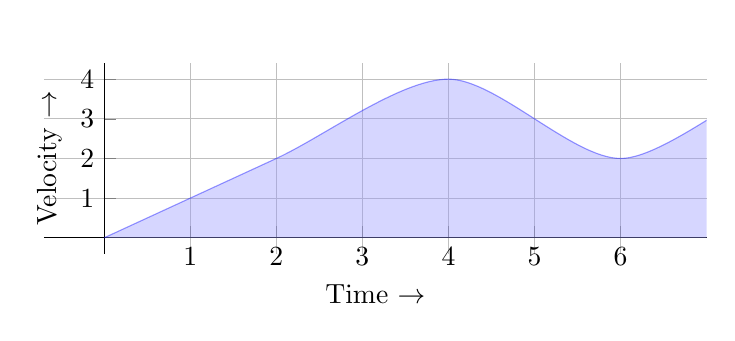
\begin{tikzpicture}
                \begin{axis}[width=10cm, height=4cm, x axis line style={}, grid =
                    major, y axis line style={},
                     title={\textbf{}}, xlabel={Time $\rightarrow$}				, xtick = {0,1,2,3,4,5,6} , xmax=7, axis lines*=center,
                     ytick={0,1,2,3,4,5,6}, ylabel={Velocity $\rightarrow$},
                     xlabel near ticks, ylabel near ticks] \addplot [color=blue, smooth,
                     domain = 0:5, fill = blue!40!white, opacity=0.4 ] coordinates {
                     (0,0) (2,2) (4,4) (6,2) (8,4) (8,0)};
                \end{axis}
                \end{tikzpicture}
        }
        \begin{tikzpicture}[overlay,remember picture,
                box/.style = {rounded corners},
                pin edge={-Stealth,thick, red}]
        \coordinate (ar1) at (-1,1.5);
        \coordinate (ar2) at (0,1.5);
        \node[semitransparent,
           fit=(ar1) (ar2),
           pin=right:\scriptsize{Area = distance travelled}]  {};
        \end{tikzpicture} 

        \vspace{0.5cm}
        \centering
        What should be the function's shape?
\end{frame}

\begin{frame}{Moving a particle with a \underline{fixed} acceleration}

        We accelerate and then brake

        \vspace{0.5cm}
        \scalebox{0.55}{
                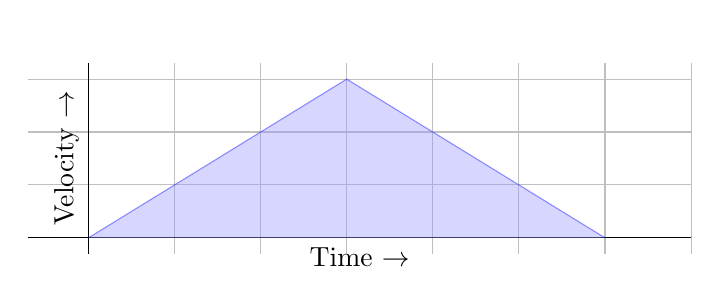
\begin{tikzpicture}
                \begin{axis}[ticks=none,width=10cm, height=4cm, x axis line style={}, grid =
                    major, y axis line style={},
                     title={\textbf{}}, xlabel={Time $\rightarrow$}, xmax=7, axis lines*=center,
                     ylabel={Velocity $\rightarrow$}] \addplot [color=blue,
                     domain = 0:5, fill = blue!40!white, opacity=0.4 ] coordinates {
                     (0,0) (2,2) (3,3) (4,2) (6,0)};
                \end{axis}
                \end{tikzpicture}
        }
        \hspace{0.6cm}
        \scalebox{0.55}{
                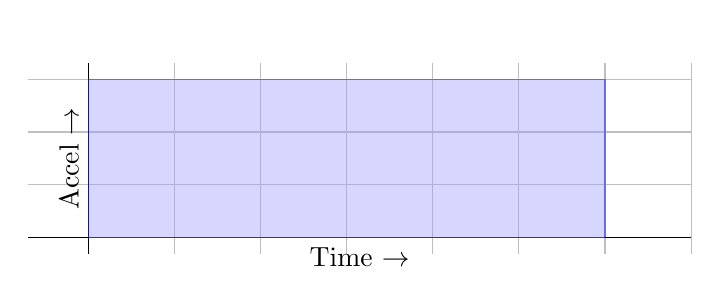
\begin{tikzpicture}
                \begin{axis}[ticks=none, width=10cm, height=4cm, x axis line style={}, grid =
                    major, y axis line style={},
                     title={\textbf{}}, xlabel={Time $\rightarrow$}				
                     , xmax=7, axis lines*=center,
                     ylabel={Accel $\rightarrow$},
                     xlabel near ticks, ylabel near ticks] \addplot [color=blue,
                     domain = 0:5, fill = blue!40!white, opacity=0.4 ] coordinates {
                     (0,0) (0,3) (2,3) (3,3) (4,3) (6,3) (6,0)};
                \end{axis}
                \end{tikzpicture}
        }
        \vspace{1cm}
        \centering
        \[
        \begin{cases}
                \mathrm{dist} = \frac{1}{2} \cdot b \cdot h \\
                h = \frac{1}{2} \cdot b \cdot \mathrm{accel}
        \end{cases}
        \Longrightarrow
        b = \sqrt{ \frac{4 \cdot \mathrm{dist}}{\mathrm{accel}} }
        \]
\end{frame}
\begin{frame}{Moving a particle with positive velocity}

        We maintain velocity and then brake

        \vspace{0.5cm}
        \scalebox{0.55}{
                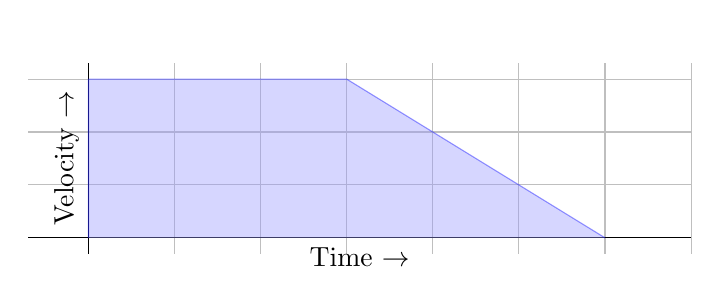
\begin{tikzpicture}
                \begin{axis}[ticks=none,width=10cm, height=4cm, x axis line style={}, grid =
                    major, y axis line style={},
                     title={\textbf{}}, xlabel={Time $\rightarrow$}, xmax=7, axis lines*=center,
                     ylabel={Velocity $\rightarrow$}] \addplot [color=blue,
                     domain = 0:5, fill = blue!40!white, opacity=0.4 ] coordinates {
                     (0,0) (0,3) (2,3) (3,3) (4,2) (6,0)};
                \end{axis}
                \end{tikzpicture}
        }
        \hspace{0.6cm}
        \scalebox{0.55}{
                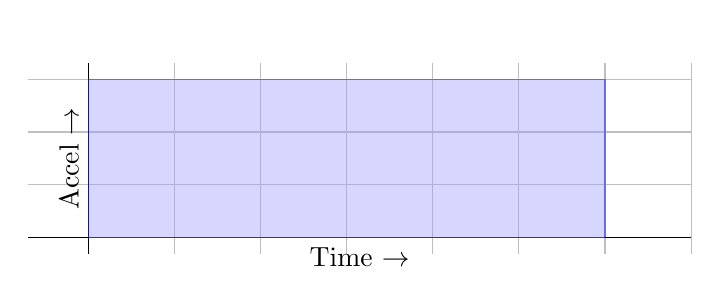
\begin{tikzpicture}
                \begin{axis}[ticks=none, width=10cm, height=4cm, x axis line style={}, grid =
                    major, y axis line style={},
                     title={\textbf{}}, xlabel={Time $\rightarrow$}				
                     , xmax=7, axis lines*=center,
                     ylabel={Accel $\rightarrow$},
                     xlabel near ticks, ylabel near ticks] \addplot [color=blue,
                     domain = 0:5, fill = blue!40!white, opacity=0.4 ] coordinates {
                     (0,0) (0,3) (2,3) (3,3) (4,3) (6,3) (6,0)};
                \end{axis}
                \end{tikzpicture}
        }
        \vspace{1cm}
        \centering
        \[
        \begin{cases}
                \mathrm{dist} = v \cdot b_1 + \frac{1}{2} \cdot v \cdot b_2 \\
                v = b_2 \cdot \mathrm{accel} 
        \end{cases}
        \Longrightarrow
        b_1 = \frac{ 2 \cdot \mathrm{dist} - \frac{v^2}{a}}{2 \cdot v}
        \]
\end{frame}
\begin{frame}{The more general case}

        We accelerate, maintain velocity, and then brake

        \vspace{0.5cm}
        \centering 
        \scalebox{0.7}{
                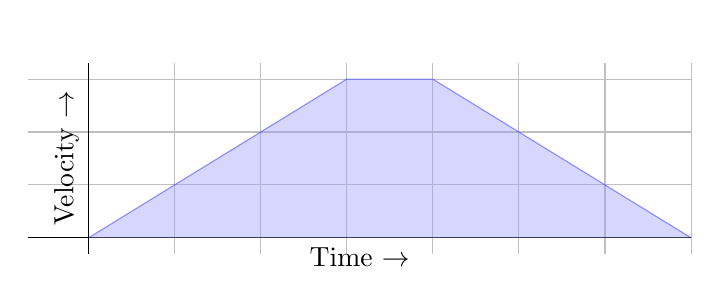
\begin{tikzpicture}
                \begin{axis}[ticks=none,width=10cm, height=4cm, x axis line style={}, grid =
                    major, y axis line style={},
                     title={\textbf{}}, xlabel={Time $\rightarrow$}, xmax=7, axis lines*=center,
                     ylabel={Velocity $\rightarrow$}] \addplot [color=blue,
                     domain = 0:5, fill = blue!40!white, opacity=0.4 ] coordinates {
                     (0,0) (1,1) (2,2) (3,3) (4,3) (5,2) (6,1) (7,0)};
                \end{axis}
                \end{tikzpicture}
        }

        \Large{\dots}
        \end{frame}

\begin{frame}{Following the leader pt. I}
  \begin{minipage}[0.3\textheight]{\textwidth}
  \begin{columns}[c]
  \begin{column}{0.45\textwidth}
   \hspace{0.3cm}
   \includegraphics[scale=0.38]{./images/fl1.png}
  \end{column}
  \begin{column}{1\textwidth}
    \includegraphics[scale=0.3]{./images/fl_plot.png}
  \end{column}
  \end{columns}
  \end{minipage}

  \pause
  Problem: Even if behind the leader in the next iteration, we might
  generate a velocity so high that we won't brake in time
\end{frame}

\begin{frame}{Following the leader pt. II}
  \begin{minipage}[1\textheight]{\textwidth}
  \begin{columns}[c]
  \begin{column}{0.45\textwidth}
          \hspace{0.4cm} 
          \includegraphics[scale=0.32]{./images/newcode.png}
  \end{column}
  \begin{column}{1\textwidth}
    \includegraphics[scale=0.3]{./images/newplot.png}
  \end{column}
  \end{columns}
  \end{minipage}

  \pause
  \vspace{0.5cm}
  Conditional arises from \alert{solving} the equation for $t$
  \[
        x_0 + v_0t + \frac{1}{2}(-2)t^2 = y_0 + 10t\ 
  \]
  No solutions, means no collisions!!
\end{frame}

\section{Conclusions}

\begin{frame}{Conclusions}

        Studied fundamentals of program semantics

        Visited a zoo of hybrid programs -- which improved our ability to
        recognise them in the wild

        Saw how to design hybrid programs \alert{formally}

        \vspace{0.5cm}
        \pause
        What next?
\end{frame}

\begin{frame}{Scenarios we did not cover}
        Movement in $n$-dimensions

        Trajectory correction

        Orbital dynamics

        \dots
\end{frame}

\begin{frame}{Open Challenges}

        Integration of uncertainty, concurrency, and communication

        A logical verification framework

        A proper handle of exact real-number computation
\end{frame}

\end{document}

